%%%%%%%%%%%%%%%%%%%%%%%%%%%%%%%%%%%%%%%%%%%%%%%%%%%%%%%%%%%%
%%  This Beamer template was created by Matteo Rucco..
%%  Anyone can freely use or modify it for any purpose
%%  without attribution.
%%
%%  Last Modified: December 7, 2014
%%

\documentclass[xcolor=x11names,compress, 
					%handout %rimuove i pause
]{beamer}

%% General document %%%%%%%%%%%%%%%%%%%%%%%%%%%%%%%%%%
\usepackage{graphicx}
\usepackage{tikz}
\usetikzlibrary{decorations.fractals}
%%%%%%%%%%%%%%%%%%%%%%%%%%%%%%%%%%%%%%%%%%%%%%%%%%%%%%


%% Beamer Layout %%%%%%%%%%%%%%%%%%%%%%%%%%%%%%%%%%
\useoutertheme[subsection=false,shadow]{miniframes}
\useinnertheme{default}
\usefonttheme{serif}
\usepackage{palatino}
\usepackage{setspace,textcomp,soul}

\setbeamerfont{title like}{shape=\scshape}
\setbeamerfont{frametitle}{shape=\scshape}
\definecolor{bluUnicam}{RGB}{27,43,74}
\definecolor{redUnicam}{RGB}{219,0,36}
\definecolor{orangeUnicam}{RGB}{234,114,40}
\setbeamercolor*{lower separation line head}{bg=redUnicam} 
\setbeamercolor*{normal text}{fg=bluUnicam,bg=white} 
\setbeamercolor*{alerted text}{fg=red} 
\setbeamercolor*{example text}{fg=black} 
\setbeamercolor*{structure}{fg=orangeUnicam} 
\setbeamercolor*{frametitle}{fg=redUnicam}


\setbeamercolor*{palette tertiary}{fg=orangeUnicam,bg=bluUnicam} 
\setbeamercolor*{palette quaternary}{fg=black,bg=black!10} 

\setbeamercovered{transparent}

\theoremstyle{definition} \newtheorem{esempio}{Esempio}
\theoremstyle{definition}
\newtheorem{definizione}{Definition} \theoremstyle{plain}
\newtheorem{teorema}{Theorem}


\begin{document}


%%%%%%%%%%%%%%%%%%%%%%%%%%%%%%%%%%%%%%%%%%%%%%%%%%%%%%
%%%%%%%%%%%%%%%%%%%%%%%%%%%%%%%%%%%%%%%%%%%%%%%%%%%%%%
\section{\scshape}
	\begin{frame}
		\title{\color{redUnicam}{Tool CNN per analisi e predizione di crisi epilettiche}}
		\begin{center}
			\author[shortname]{\textbf{Manuel Cretone, Emilio Silvestri\\Tutor: prof Marco Piangerelli}\\
			\fontsize{8pt}{10}\selectfont{Group project}
			\institute[shortinst]{\fontsize{6pt}{6}\selectfont{\inst{1}University of Camerino, Italy}}}
			\date{
				\begin{figure}[htpb!]
				\centering{
			  		
\includegraphics[width=0.20\textwidth]{immagini/stemma}
				 }
				\end{figure}
			}
		\titlepage
		\end{center}
	\end{frame}

%%%%%%%%%%%%%%%%%%%%%%%%%%%%%%%%%%%%%%%%%%%%%%%%%%%%%%
%%%%%%%%%%%%%%%%%%%%%%%%%%%%%%%%%%%%%%%%%%%%%%%%%%%%%%
%{
%%\usebackgroundtemplate{\includegraphics[width=\paperwidth,height=\paperheight]{./immagini/camerino}}
%\begin{frame}{Computer Science @ Unicam}
%
%The Unicam Group - Formal Methods and Analysis of Complex Systems :
%\begin{itemize}
%\item Professor and TOPDRIM coordinator: E. Merelli http://www.cs.unicam.it/merelli/BioShape-lab/
%\item Researcher: L. Tesei
%\item PhD Students: N. Paoletti, M. Taffi, P. Penna and M. Piangerelli
%\item Students (Bachelor and Master): J. Binchi (joint work with ISI), J. De Berardinis (TDA comparison)
%\end{itemize}
%\end{frame}
%
%}
%%%%%%%%%%%%%%%%%%%%%%%%%%%%%%%%%%%%%%%%%%%%%%%%%%%%%%
%%%%%%%%%%%%%%%%%%%%%%%%%%%%%%%%%%%%%%%%%%%%%%%%%%%%%%
\begin{frame}{Outline}
	\tableofcontents
\end{frame}


\section{Introduzione}
		
	\subsection{Epilessia}
		\begin{frame}{\subsecname}
			Malattia neurologica che colpisce 50 milioni di persone nel mondo.
			
			 Caratterizzata da specifici eventi clinici: crisi epilettiche
			\begin{itemize}
				\item Alterazione del normale funzionamento dell'encefalo
				\item Tipi di crisi epilettiche:
				 \begin{itemize}
				 	\item Parziali: una singola parte
				 	\item Generalizzate: entrambi gli emisferi
				 \end{itemize}
			\end{itemize}
		\end{frame}
		
	%\subsection{EEG e edf}
		\begin{frame}{EEG e EDF}
			Diagnosi epilessia tramite analisi elettroencefalogramma
			
			Segnali generati dalla differenza di potenziale degli elettrodi applicati allo scalpo
			
			\begin{itemize}
				\item Registra attività elettrica dell'encefalo
				\item Riproduce segnali su tracciati grafici
			\end{itemize}
			
			Uso di file .edf (European Data Format) 
			\begin{itemize}
				\item Archiviazione dei segnali registrati
				\item Caratteristiche della registrazione (frequenza di campionamento, durata...)
			\end{itemize}
		\end{frame}
	
	\subsection{Il progetto: obiettivi}
		\begin{frame}{\subsecname}
			\begin{figure}
				
\includegraphics[scale=0.3]{immagini/prova3-piccolo}
			\end{figure}
			
			Il programma realizzato ha tre scopi principali:\pause
			\begin{itemize}
				\item Offrire una visione grafica di file .edf contenenti tracciati elettroencefalografici \pause
				\item Ridurre la fase di individuazione di crisi epilettiche all'interno di un tracciato EEG \pause
				\item Offrire un ambiente di allenamento di reti neurali personalizzate per l'individuazione di crisi epilettiche
			\end{itemize}
		\end{frame}
		
	\subsection{Workflow progetto}
		\begin{frame}{\subsecname}
			\begin{itemize}
				\item studio EEG e crisi epilettiche\pause
				\item studio teorico CNN\pause
				\item studio tool di sviluppo\pause
				\item creazione di un dataset di allenamento bilanciato\pause
				\item creazione e allenamento rete per le predizioni\pause
				\item costruzione di architettura web backend e frontend
			\end{itemize}
		\end{frame}
	
	
\section{Reti Neurali}	
	\subsection{Reti Neurali}
		\begin{frame}{\subsecname: Overview}
			\begin{figure}
				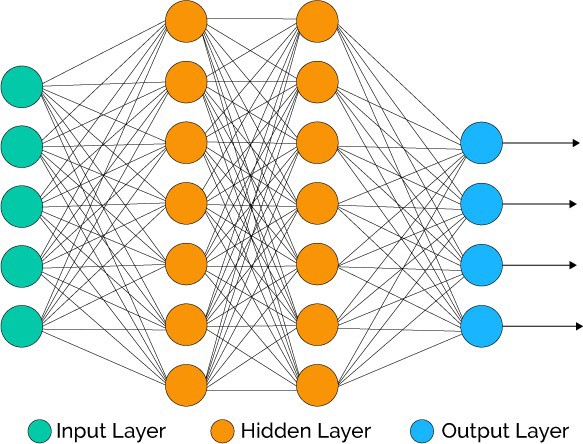
\includegraphics[scale=0.3]{immagini/linear}
			\end{figure}
			\begin{itemize}
				\item Modelli computazionali basati su neuroni
				\item Ispirate al funzionamento biologico del cervello
				\item Applicate nella risoluzione di problemi ingegneristici, informatici, di simulazione...
			\end{itemize}
		\end{frame}
		
		\begin{frame}{\subsecname: Overview}
			Funzionamento neurone:
			\begin{itemize}
				\item Una o più connessioni in ingresso e uscita
%				\item Il segnale trasmesso tra due neuroni è un numero reale, moltiplicato per il peso della connessione
				\item Somma dei segnali in ingresso moltiplicati per i pesi delle connessioni
				\item Aggiunta di un eventuale \textit{bias}
				\item Funzione di attivazione e segnale in uscita
			\end{itemize}
			
			Tipologie di rete:
			\begin{itemize}
				\item Feedforward: layer di neuroni con connessioni in una sola direzione
				\item Ricorsive: connessioni con neuroni dello stesso livello o all'indietro
			\end{itemize}
		\end{frame}
		
		\begin{frame}{\subsecname: Training}
				\textbf{Tipologie di allenamento:}
				\begin{itemize}
					\item Supervised Learning\pause
					\item Unsupervised Learning\pause
					\item Semi-supervised Learning\pause
					\item Apprendimento per rinforzo
				\end{itemize}\pause
			\begin{columns}
				\begin{column}{0.7\textwidth}
					\textbf{Passi allenamento supervisionato:}
					\begin{itemize}
						\item Inizializzazione\pause
						\item Feed-forward\pause
						\item Loss function\pause $\rightarrow$ Calcolo errore\pause
						\item Differentiation\pause $\rightarrow$ Diminuzione loss\pause
						\item Backpropagation e weights update
					\end{itemize}\pause
				\end{column}
				\begin{column}{0.3\textwidth}
					\begin{center}
						Ripetuti per ogni \textit{epoca}\\
						Validation e Test
					\end{center}
				\end{column}
			\end{columns}
		\end{frame}
	
	\subsection{Reti Neurali Convoluzionali}
		\begin{frame}{\subsecname}
			\begin{itemize}
				\item Adatte ad input di grandi dimensioni\pause
				\item Riconoscimento di \textit{pattern} nell'architettura\pause
				\item Applicazione di \textit{kernel} per individuazione di features nei dati
			\end{itemize}
			\begin{figure}
				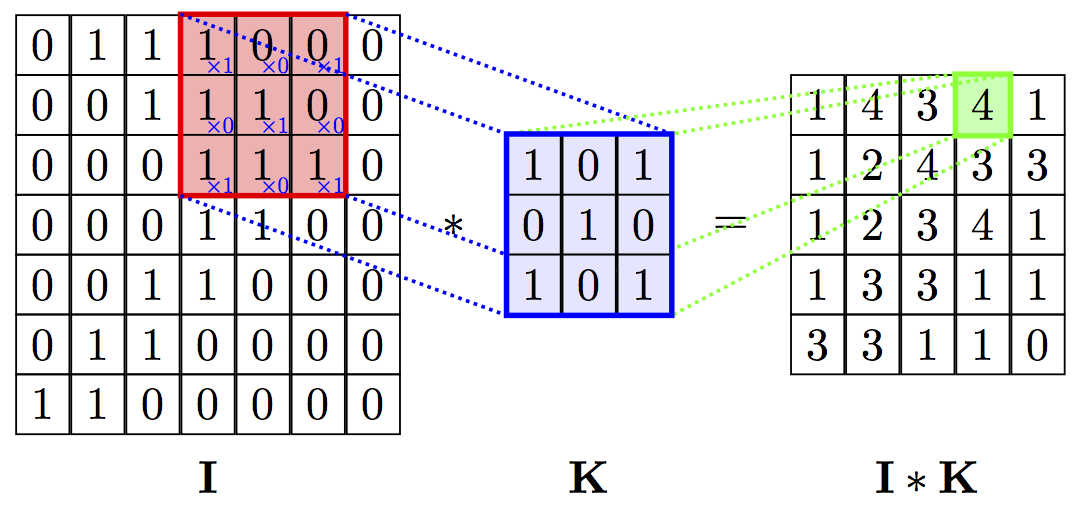
\includegraphics[scale=0.9]{immagini/convolution}
			\end{figure}
		\end{frame}
		\begin{frame}{\subsecname}
			Parametri layer convoluzionale:
			\begin{itemize}
				\item Input (I)
				\item Profondità (K)
				\item Stride (S)
				\item Zero-Padding (P)
			\end{itemize}\pause
			\begin{center}
				\textbf{Dimensione del volume di output}:
				\begin{equation}
					O={\frac{(I - K - 2P)}{S} +1}
				\end{equation}
			\end{center}
		\end{frame}
		\begin{frame}{\subsecname}
			\begin{figure}
				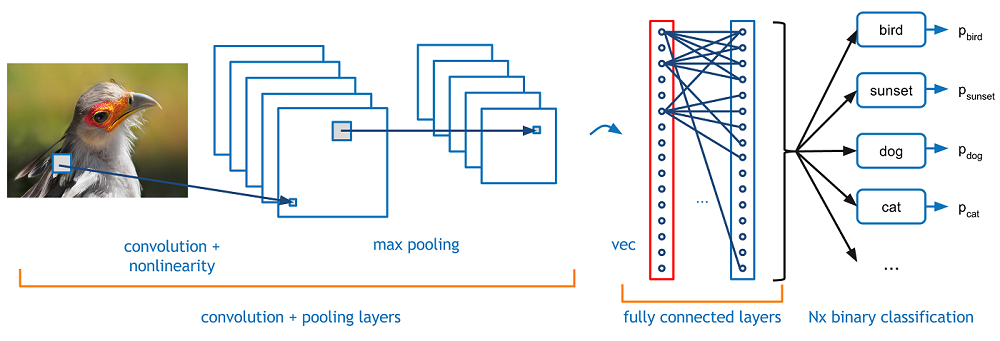
\includegraphics[width=0.8\textwidth]{immagini/cnnlayer}
			\end{figure}
			\begin{itemize}
				\item Convolutional layers
				\item Pooling Layers (max, average...)
				\item Fully Connected Layers
			\end{itemize}
		\end{frame}
		\begin{frame}{Convoluzioni 1D}
			\begin{figure}
				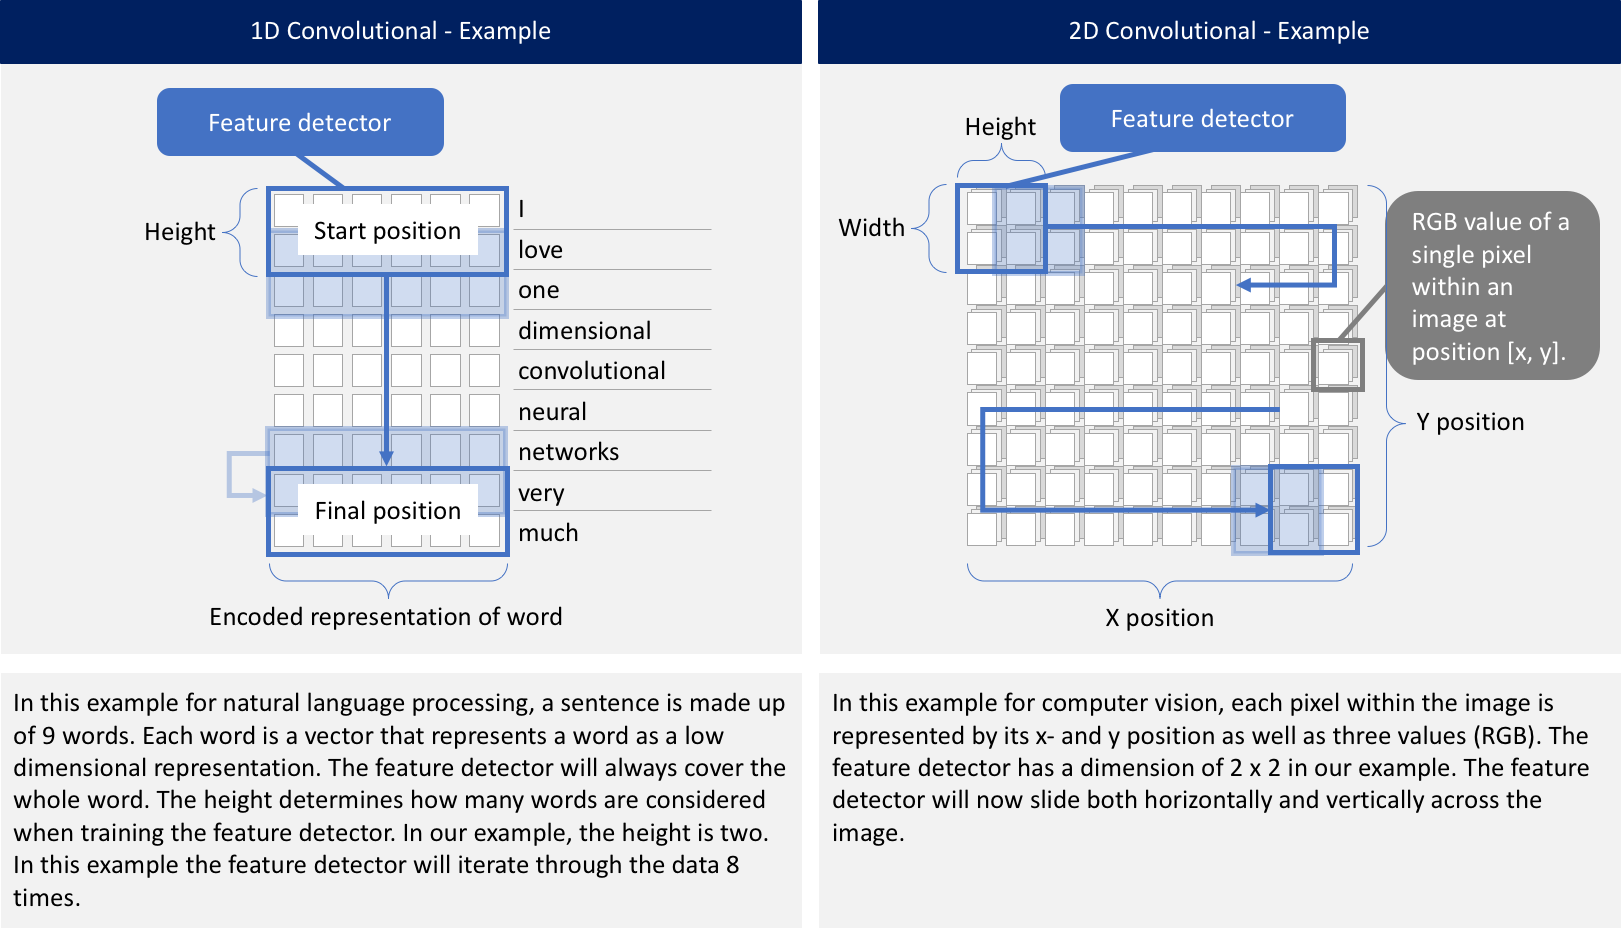
\includegraphics[width=0.7\textwidth]{immagini/conv1d}
			\end{figure}
			\begin{columns}
				\begin{column}{0.5\textwidth}
					Conv 1D (segnali, NLP...)
					\begin{itemize}
						\item Input bidimensionale\\\textit{(C, W)}
						\item Il kernel scorre lungo la dimensione W
					\end{itemize}
				\end{column}
				\begin{column}{0.5\textwidth}
					Conv 2D (immagini)
					\begin{itemize}
						\item Input tridimensionale\\\textit{(C, H, W)}
						\item Il kernel scorre lungo le dimensioni H e W
					\end{itemize}
				\end{column}
			\end{columns}
		\end{frame}
		\begin{frame}{Modello proposto}
			\begin{figure}
				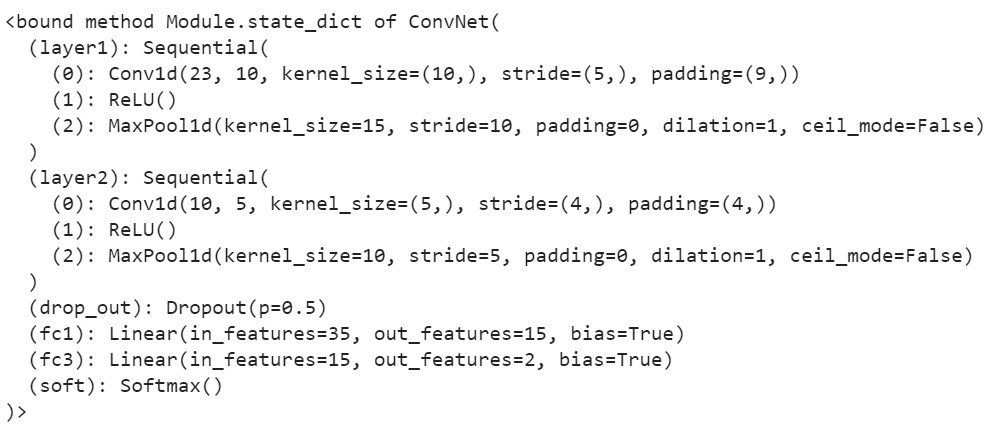
\includegraphics[width=1\textwidth]{immagini/ourcnn}
			\end{figure}\pause
			\begin{columns}
				\begin{column}{0.5\textwidth}
					\begin{itemize}
						\item Sequential:\pause
						\begin{itemize}
							\item Convolution\pause
							\item ReLU activation\pause
							\item MaxPool\pause
						\end{itemize}
					\end{itemize}
				\end{column}
				\begin{column}{0.5\textwidth}
					\begin{itemize}
						\item Dropout\pause
						\item Fully-connected\pause
						\item Softmax
					\end{itemize}
				\end{column}
			\end{columns}
		\end{frame}
		
\section{Training}
	\subsection{Dataset}
		\begin{frame}{\subsecname}
			\begin{figure}
				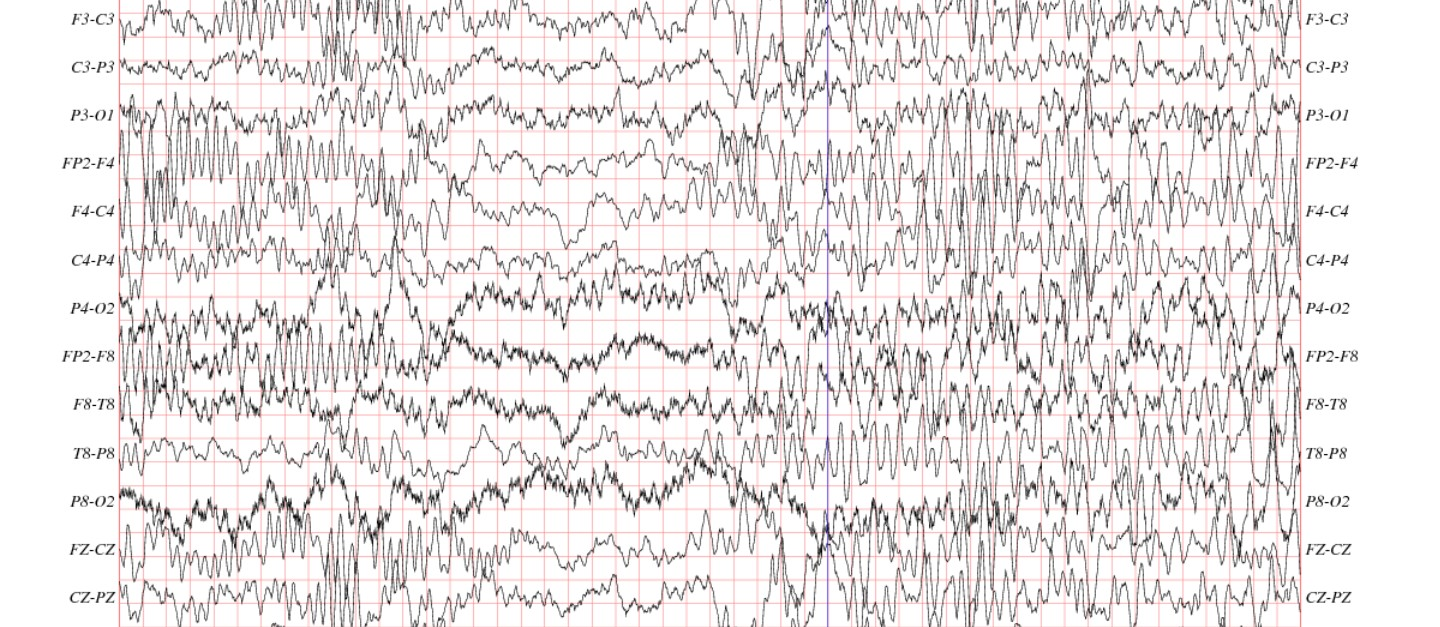
\includegraphics[width=0.9\textwidth]{immagini/chb}
			\end{figure}
			\begin{itemize}
				\item Children's Hospital Boston database (22 pazienti totali)
				\item Pazienti 1,2,3,5,7 e 8
				\item File con almeno un evento di crisi
				\item Frequenza di campionamento 256Hz
				\item 23 canali di campionamento
			\end{itemize}
		\end{frame}
		\begin{frame}{Training della rete}
			\begin{itemize}
				\item\textbf{Preparazione del dataset:}
				\begin{itemize}
					\item Isolamento dei segnali di crisi
					\item Suddivisione in finestre da 30 secondi, con stride di 1
					\item Eliminazione segnali pre e post ictali (5 minuti)
					\item Selezione finestre non di crisi
				\end{itemize}
				\item \textbf{Training:}
					\begin{itemize}
						\item 30 epoche
						\item Cross Entropy Loss $loss(x, class) 
								%= -log(exp(x[class]) / (\sum_j exp(x[j])))
               				= -x[class] + log(\sum_j exp(x[j]))$
						\item Adam Optimizer (Adaptive moment estimation)
					\end{itemize}
				\item\textbf{Validazione}: 80\% training set, 20\% validation set\\
				\item\textbf{Test} su file esterni al training set
			\end{itemize}
		\end{frame}
	

\section{Tecnologie}
	\subsection{Backend}
		\begin{frame}{\subsecname}
			\begin{itemize}
				\item Python
				\item Django Web Framework 
				\item PyTorch 
				\item PyEdflib
			\end{itemize}
			\begin{figure}
				
\includegraphics[width=0.3\textwidth]{immagini/python}
				
\includegraphics[width=0.3\textwidth]{immagini/django}
				
\includegraphics[width=0.5\textwidth]{immagini/pytorch}
			\end{figure}
		\end{frame}
	
	\subsection{Frontend}
		\begin{frame}{\subsecname}
			\begin{itemize}
				\item Angular
				\item Ionic
				\item Highcharts 
			\end{itemize}
			\begin{figure}
				
\includegraphics[width=0.2\textwidth]{immagini/angular}
				
\includegraphics[width=0.4\textwidth]{immagini/ionic}
				
\includegraphics[width=0.7\textwidth]{immagini/highcharts}
			\end{figure}
		\end{frame}


\section{Il software}
	\begin{frame}{\secname}
		\begin{itemize}
			\item Tool Analisi
			\item Tool Predizione
			\item Tool Training
		\end{itemize}
	\end{frame}
	\subsection{Tool analisi}
		\begin{frame}{\subsecname}
			\begin{figure}
				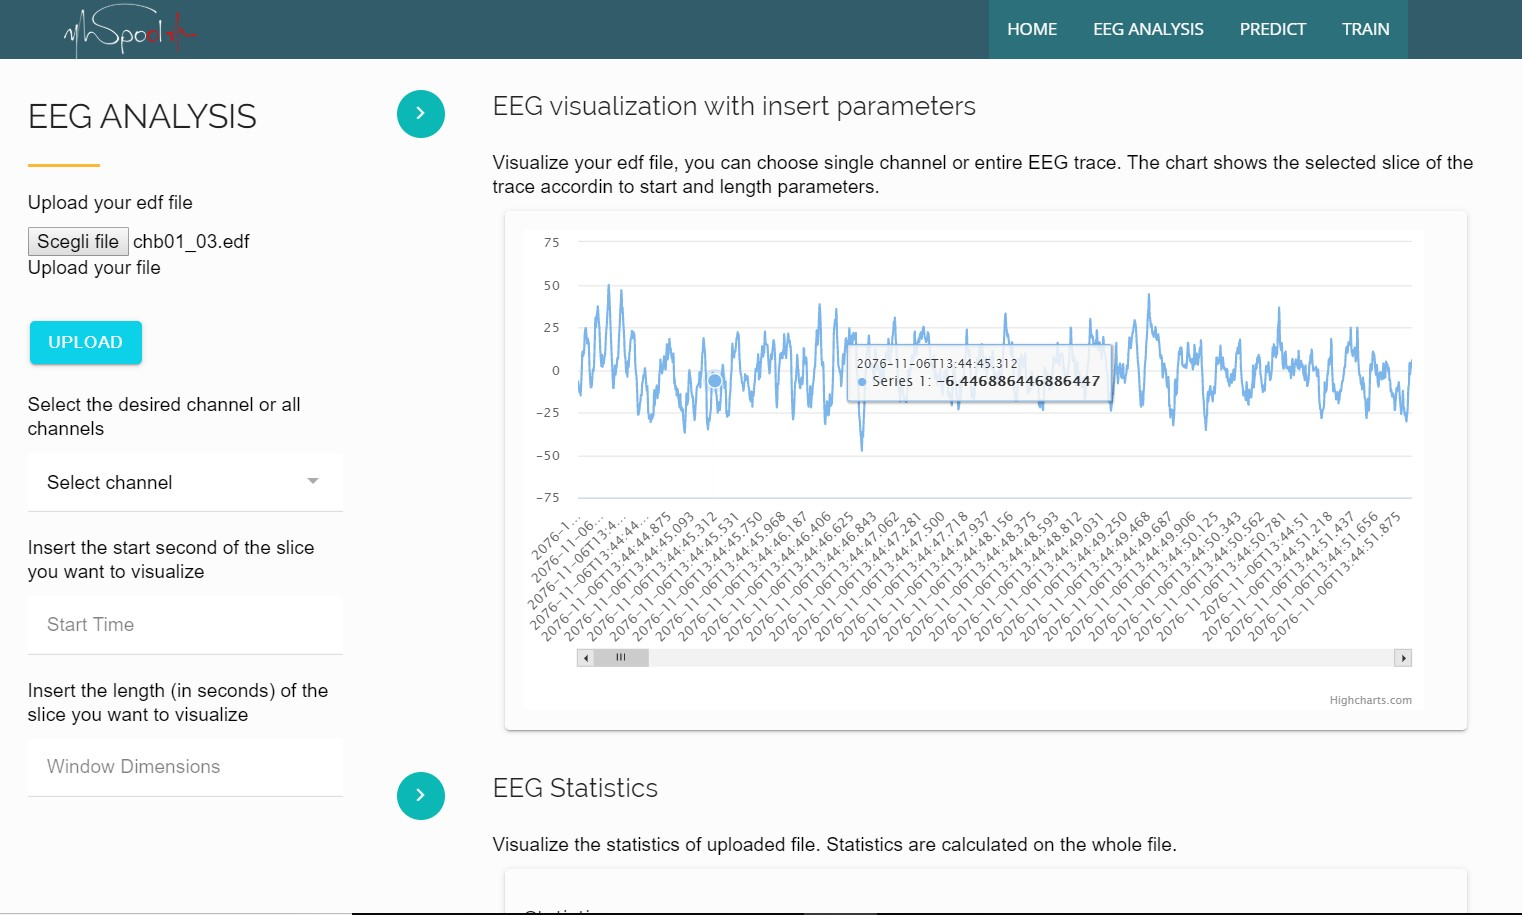
\includegraphics[width=0.8\textwidth]{immagini/analysis1}
			\end{figure}
			Servizi offerti:
			\begin{itemize}
				\item Visualizzazione EEG singolo canale / intero tracciato
				\item Statistiche intero file 
				\item Visualizzazione grafico distribuzione valori
			\end{itemize}
		\end{frame}
	
	\subsection{Tool predizione}
		\begin{frame}{\subsecname}
			\begin{figure}
				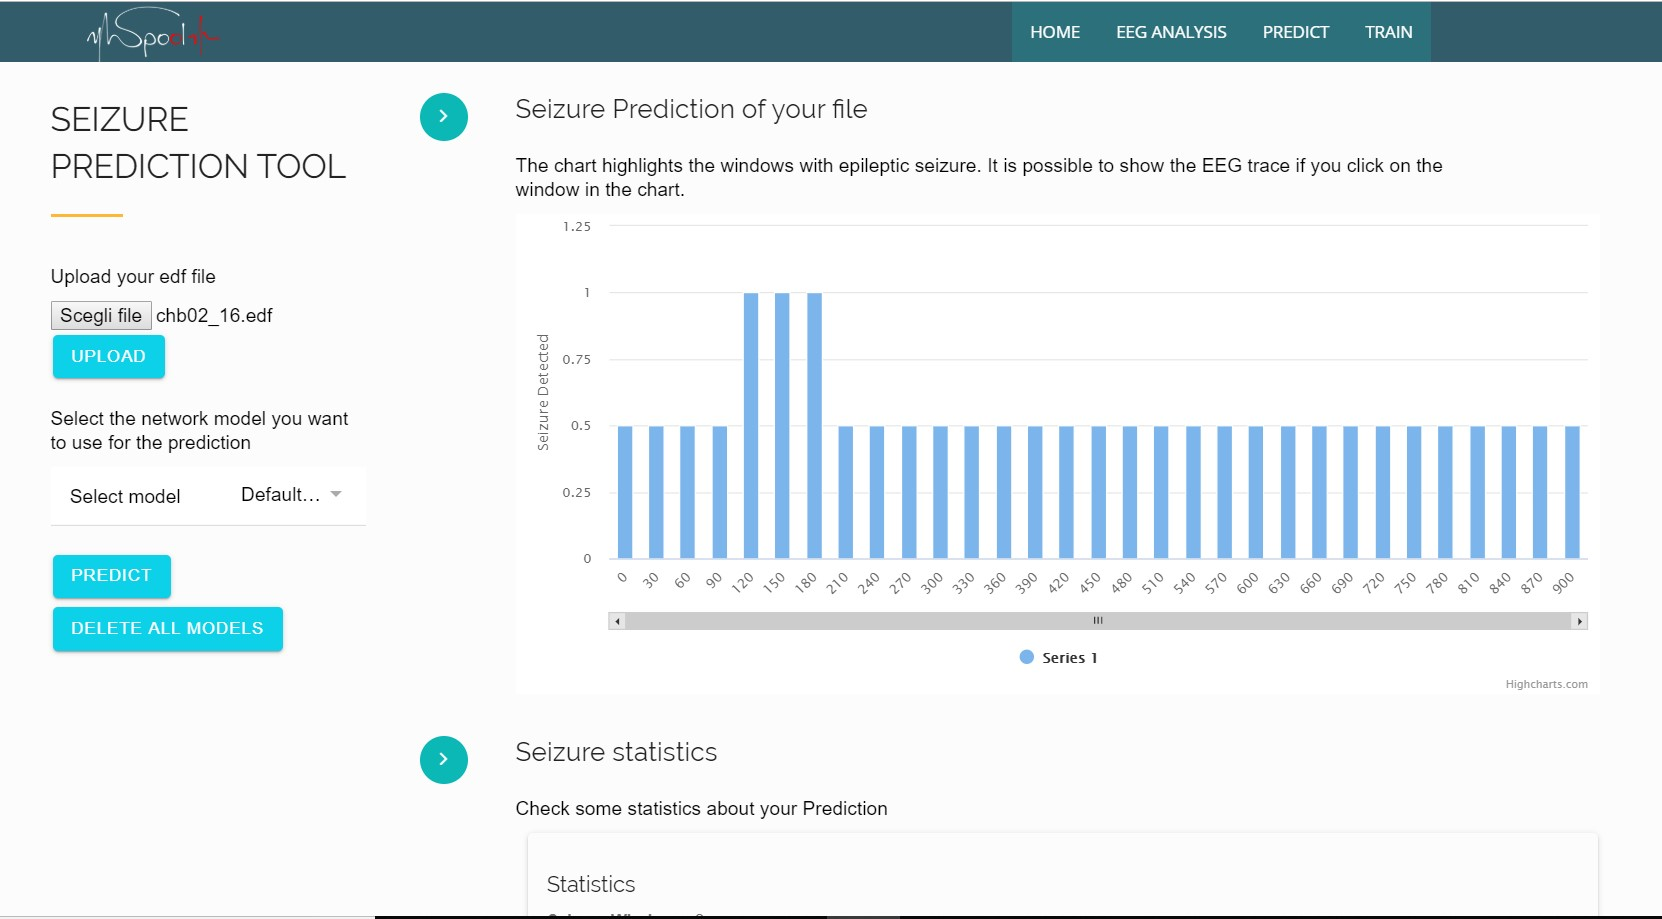
\includegraphics[width=0.8\textwidth]{immagini/prediction1}
			\end{figure}
			Servizi offerti:
			\begin{itemize}
				\item Visulizzazione predizione crisi per ogni finestra
				\item Statistiche predizione
				\item Grafico EEG finestra selezionata 
			\end{itemize}
		\end{frame}
	
	\subsection{Tool training}
		\begin{frame}{\subsecname}
			\begin{figure}
				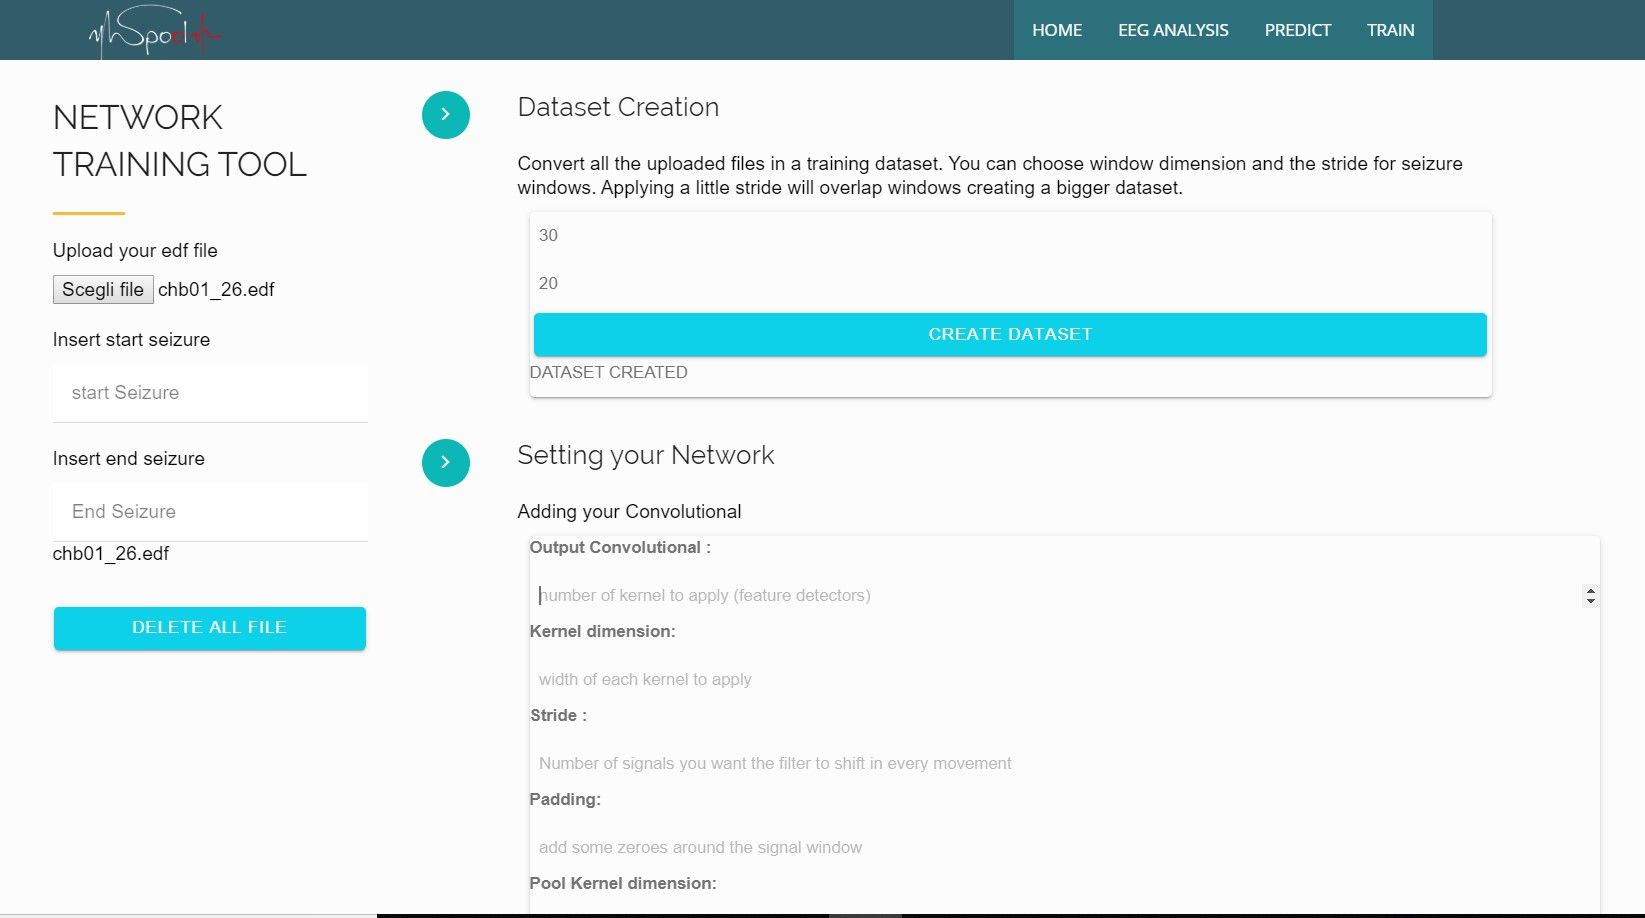
\includegraphics[width=0.8\textwidth]{immagini/training1}
			\end{figure}
			Servizi offerti:
			\begin{itemize}
				\item Inserimento file di training e creazione dataset
				\item Creazione rete personalizzata
				\item Training della rete creata
			\end{itemize}
		\end{frame}
		
		



\section*{Conclusioni}
	\begin{frame}{Vantaggi}
		\begin{itemize}
			\item visualizzazione tracciati EEG
			\item calcolo statistiche su EEG
			\item predizione di crisi epilettiche attraverso reti neurali preallenate
			\item creazione rete neurale personalizzata e predizione
		\end{itemize}
	\end{frame}

	\begin{frame}{Sviluppi futuri}
		\begin{itemize}
			\item Analisi di diversi tipi di file (.csv, .txt...)
			\item Deployment su server remoto\pause
			\item Maggiore personalizzazione delle reti \pause
			\item Ottimizzazione e diversificazione delle reti pre-allenate offerte
		\end{itemize}
	\end{frame}
	
	\begin{frame}
		\begin{center}
			
\includegraphics[width=6.5cm]{./immagini/thanks}
		\end{center}
	\end{frame}

\end{document}
